\section{Simulation Results}
\label{sec:simulation}

To demonstrate the feasibility of SemiAIM as well as evaluate the
hypothesis that SemiAIM can offer substantial improvements over
traffic signals and FCFS-Signal, we modified the AIM4 simulator at
\url{http://www.cs.utexas.edu/~aim} to simulate the behavior of
vehicles in the constraint-based reservation system and measured the
average delays of vehicles under (1) AIM, (2) SemiAIM, and (3) traffic
signals with optimized signal timing. In all experiments,
we spawn vehicles in each lane according to a Poisson distribution with the
expectation of 360 vehicles per hour. We denote this setting as
traffic level = 360 vehicles/hour/lane.\footnote{We choose this
traffic level as being high enough to cause significant delays at
signals, but light enough to allow for benefits even if cars are not
precisely controlled. Figure~\ref{fig:figure5} examines higher traffic
levels.} We assume the intersection is fully observable to the intersection
manager.

We expect that in the presence of semi-autonomous vehicles, SemiAIM
will provide significant advantages over FCFS-Signal if we assume that
semi-autonomous vehicles have to act as fully human-driven vehicles in
FCFS-Signal.  However, we do not expect that semi-autonomous traffic
under SemiAIM will perform as well as fully autonomous traffic in AIM.
The goal of SemiAIM is not to replace AIM, but rather to provide many
of its benefits prior in the time period between today, when most cars
are driven fully manually, and the time when all cars are fully
autonomous.  To do so, it leverages features of semi-autonomy, that we
expect will be widespread much sooner than full autonomy.

The implementation of autonomous vehicles (Type A) and human-driven
vehicles (Type H) can be referenced from
\cite{bib:Dresner08Multiagent}. The semi-autonomous vehicles can be
implemented according to their description in
Section~\ref{sec:vehicles}. The concrete implementation is as follows.

\begin{enumerate}

\item{Type SA-ACC: IM tries to reserve the tiles the vehicle needs to
occupy directly following the vehicle in front of it, if they are
heading for same destination lane. If tiles successfully reserved,
IM grants confirmation, otherwise rejects.}

\item{Type SA-CC: IM tries to reserve the tiles the vehicle needs to
occupy if it moves in constant velocity and not making a turn. If
tiles successfully reserved, IM grants confirmation, otherwise
rejects.}
 
\item{Type SA-Com: IM tries to reserve ALL the tiles in the trajectory
that a vehicle would occupy. If tiles successfully reserved, IM
grants confirmation, otherwise rejects.}

\end{enumerate}

We experimentally generated the \emph{optimized} traffic signal phase
plan in Table~\ref{table:phase} by using randomized greedy search in
the parameters space with random restart.  According to this plan,
there is a 30 second green phase for traffic coming from East and
West, followed by a 3 second yellow phase and a 5 second red
phase. Then, there is a 8 second green phase for traffic from South
direction only, followed by a 3 second yellow phase and a 5 second red
phase, etc.

% \commentp{how was this plan arrived at?  Why isn't it symmetric? (why 30s for East-West but 40s for North-South?)}

\begin{table}
\caption{The traffic signal phase plan.}
\label{table:phase}
\centering
\begin{tabular}{|l|c|c|c|}
\hline
Direction & Green Phase & Yellow Phase & Red Phase \\
\hline
  East-West & 30s & 3s & 5s \\
  South & \ 8s & 3s & 5s \\
  East & 10s & 1s & 5s \\
  North-South & 40s & 3s & 5s \\
  West & 10s & 1s & 5s \\
  North & \ 8s & 3s & 5s \\
\hline
\end{tabular}
\end{table}

The experiments were conducted in a $3 \times 3$ intersection (3 lanes
in each direction) as shown in Figure~\ref{fig:demo}.  In all cases,
we measure the average vehicle delay, where delay is computed as the
increase in travel time compared to traversing the intersection
without slowing down at all, as if no other vehicles were on the
road. Thus, lower delays correspond to better performance.  This
measure is the same one used in \cite{bib:Dresner08Multiagent}. For
all the vehicles, both the static buffer and the edge time buffer are
0.25 meters (see \cite{bib:Dresner08Multiagent} for details), when
auto-controlled.

% No such constraint is relevant to human-driven
% vehicles.\commentp{I don't think that last sentence is needed - unless
% it becomes a part of the official protocol for semi-autonomous
% vehicles.} \commentn{I think I can just delete it.}

In the first experiment, the traffic consisted of all five types of
vehicles we defined in Section~\ref{sec:vehicles}. The results are in
Figure~\ref{fig:figure2}. The experiments only compare two types of
vehicles at the same time---human-driven vehicles (Type H) and the
type of vehicles specified in the legends. We gradually increased the
percentage of (semi-)autonomous vehicles while keeping the traffic
level at 360 vehicles/hour/lane.

For example, for the line of Type SA-ACC vehicles, at origin point,
there are 0\% SA-ACC vehicles and 100\% human-driven vehicles. At the
point of ratio = 1, there are 100\% SA-ACC vehicles and 0\%
human-driven vehicles. At the point of ratio = 0.4, there are 40\%
SA-ACC vehicles and 60\% human-driven vehicles. As described in the
legend, the traffic level is 360 vehicles/hour/lane, so it can be
easily calculated how many vehicles of a certain type are spawned in
each lane.

It can be observed that semi-autonomous vehicles with more features have better
performance---this is shown in Table~\ref{table:type}. For example,
SA-ACC vehicles have three features, while SA-CC only have two.
Now we want to examine how semi-autonomous vehicles attribute
their performance to each feature they have. Therefore, in
Figure~\ref{fig:figure1}, we isolate the features for different types
of semi-autonomous vehicles and only consider one at a time. From this
perspective, Figure~\ref{fig:figure2} make a comparison between sets of
features, while Figure~\ref{fig:figure1} compares features themselves.

The setup of this experiment is the same as Figure~\ref{fig:figure2}, but
we only allow a certain vehicle to have one feature. For example, the
line of Adaptive Cruise Control Only, we simulate a vehicle that only
has Adaptive Cruise Control.  As can be seen, the feature of
communication device is more important than other features in terms of
reducing delay time.  It implies that being able to communicate
is fundamental to the efficiency of intersections.

% Intuitively, for a vehicle with cruise control or
% adaptive cruise control, if it misses the chance to enter
% intersection, it has to wait for the next green phase. For vehicles
% with communication devices, they could always enter when the tiles
% they required are clear.

% \commentn{I basically rewrote this part. You questioned why we use
% different legends for two figures. I also changed the order of
% Figure~\ref{fig:figure1} and Figure~\ref{fig:figure2}. The first one
% is a very obvious comparison, and the second one is comparing
% different features that semi-autonomous vehicles could have. }

% (in contrast to what's shown in Table~\ref{table:1}). 

\begin{figure}

\centering
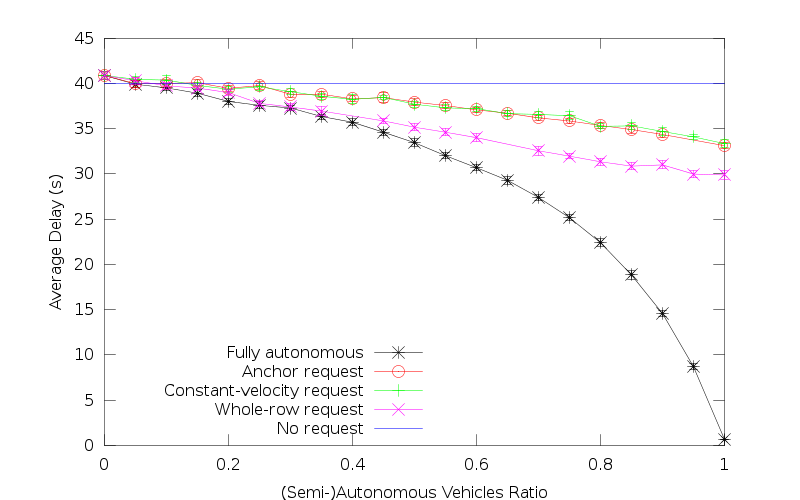
\includegraphics[width=0.8\columnwidth]{figures/figure_2.png}
\caption{(Semi-)Autonomous vehicles vs. Human-Driven vehicles, traffic
level = 360 vehicles/lane/hour. The simulation time is 1800 seconds.
Each data point is an average of the delay times over 30 runs.}
\label{fig:figure2}

\centering
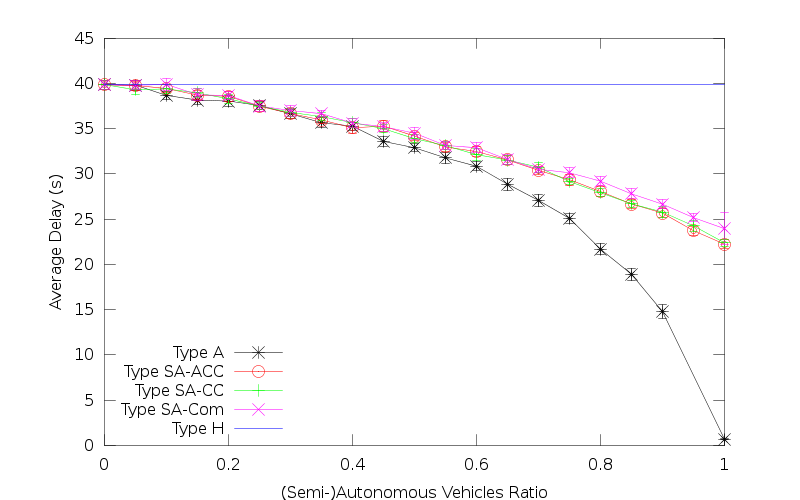
\includegraphics[width=0.8\columnwidth]{figures/figure_1.png}
\caption{Comparison on different features of semi-autonomous vehicles
, traffic level = 360 vehicles/lane/hour. The simulation time is 1800
seconds. Each data point is an average of the delay times over 30 runs.}
\label{fig:figure1}

\mbox{}

\end{figure}

% Figure~\ref{fig:figure1} shows that as the number of autonomous
% vehicles increases, the average delay decreases. In particular, when
% most vehicles are autonomous, the average delay is close to zero.  In
% the second experiment, we created a traffic consisting of
% human-controlled vehicles and two kinds of semi-autonomous vehicles
% but no autonomous vehicles.  We measured the average delay of all
% vehicles when we gradually increased the percentage of semi-autonomous
% vehicles.  Then we compared SemiAIM with optimized traffic signals.
% The results in Figure~\ref{fig:figure2} shows that as the number of
% semi-autonomous vehicles increases, the average delay decreases under
% SemiAIM.  While the decrease is not as dramatic as the decrease when
% the percentage of autonomous vehicles is near 100\% in
% Figure~\ref{fig:figure1}, SemiAIM can reduce about 43\% of the average
% delay when most vehicles are semi-autonomous.

In addition, we compared the performance in traffic with a mixture of
different types of vehicles.  We conducted two experiments to test 1)
the effect of gradually shifting from human-driven vehicles to
autonomous and semi-autonomous vehicles, and 2) the effect of shifting
from semi-autonomous vehicles to fully autonomous vehicles.  The
schedule for shifting is indicated in Tables~\ref{table:3}
and~\ref{table:4}, which can be used to interpret the mix of vehicles
along the x-axes of Figures~\ref{fig:figure3} and~\ref{fig:figure4}
respectively.

\begin{enumerate}

\item Gradually replace human-driven vehicles with semi-autonomous
  vehicles. The result shows that with appearance of more autonomous
  and semi-autonomous vehicles (i.e.\ fewer human-driven vehicles), the
  delay time decreases. The result is shown in
  Figure~\ref{fig:figure3}.

\item Gradually replace semi-autonomous vehicles with fully autonomous
  vehicles. The result shows that when the percentage of human
  vehicles is fixed, the delay time decreases with appearance
  of more autonomous vehicles (i.e.\ fewer semi-autonomous vehicles).
  The result is shown in Figure~\ref{fig:figure4}.

\end{enumerate}

The performance of semi-autonomous vehicles can be significantly
better than human-driven vehicles in small traffic levels. However,
the benefits decrease significantly at higher traffic levels.  In
Figure~\ref{fig:figure5}, we increase the traffic level to 540
vehicles/hour/lane. At this traffic level, congestion appears.  It is
true that semi-autonomy would not ``harm'' normal traffic which
follows traffic signals, but they have almost no chance to enter the
intersection in phases other than when the signal is green. This
condition leads to little or no improvement over traditional traffic
light policy.

This result confirms our hypothesis that while semi-autonomous
vehicles can significantly bridge the gap between the time when all
vehicles are human-driven to that when most are autonomous, there will
likely always remain strong benefits of full autonomy, especially at
high traffic levels.  Nevertheless, for lower levels of traffic, the
benefits of semi-autonomy can be large.

% \commentp{These tables should include a column indicating what point
% on the x-axis each row falls.} \commentn{Added.}

\begin{table}[t]
\caption{The distribution of semi-autonomous vehicles in Figure~\ref{fig:figure3}.}
\label{table:3}
\centering
\begin{tabular}{|c|c|c|}
    \hline
    Type H&  Type SA-* (x-axis)&    Type A\\
    \hline
    90&       9&    1\\
    \hline
    87&     11&    2\\
    \hline
    84&     13&    3\\
    \hline
     ...&   ...&   ...\\
    \hline
         0&     69&  31\\
    \hline
\end{tabular}

\mbox{}

\caption{The distribution of semi-autonomous vehicles in Figure~\ref{fig:figure4}.}
\label{table:4}
\centering
\begin{tabular}{|c|c|c|}
    \hline
     Type H&  Type SA-* (x-axis)&    Type A\\
    \hline
     10&     85&    5\\
    \hline
     10&     80&  10\\
    \hline
     10&     75&  15\\
    \hline
      ...&  ...&  ...\\
    \hline
        10&       5&  85\\
    \hline
\end{tabular}

\end{table}


\begin{figure}
\centering
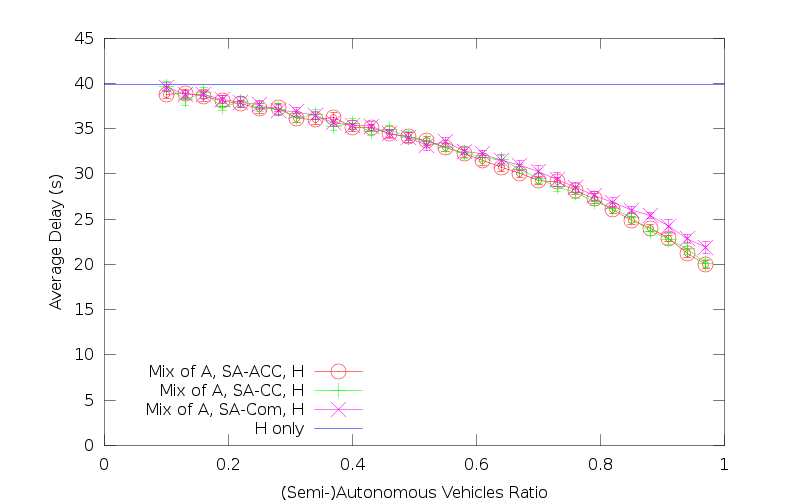
\includegraphics[width=0.8\columnwidth]{figures/figure_3.png}
\caption{The average delay time in different percentage of semi-autonomous
  vehicles and autonomous vehicles. The combination of each point is
  specified in Table \ref{table:3}. Traffic level = 360 vehicles/lane/hour.
  Simulation time is 1800 seconds.}
\label{fig:figure3}

\mbox{}

\centering
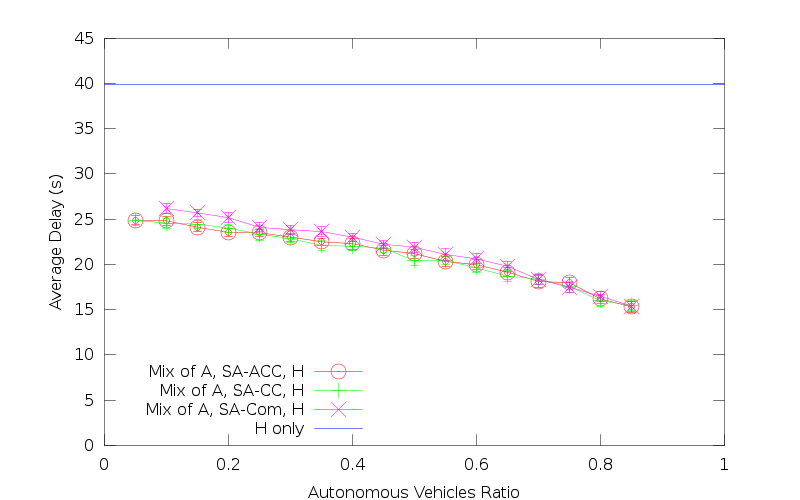
\includegraphics[width=0.8\columnwidth]{figures/figure_4.png}
\caption{The average delay time in different percentage of human
driven vehicles and semi-autonomous vehicles.  The combination of
each point is specified in Table \ref{table:3}.  traffic level = 360
vehicles/lane/hour. Simulation time is 1800 seconds.}
\label{fig:figure4}

\mbox{}

\centering
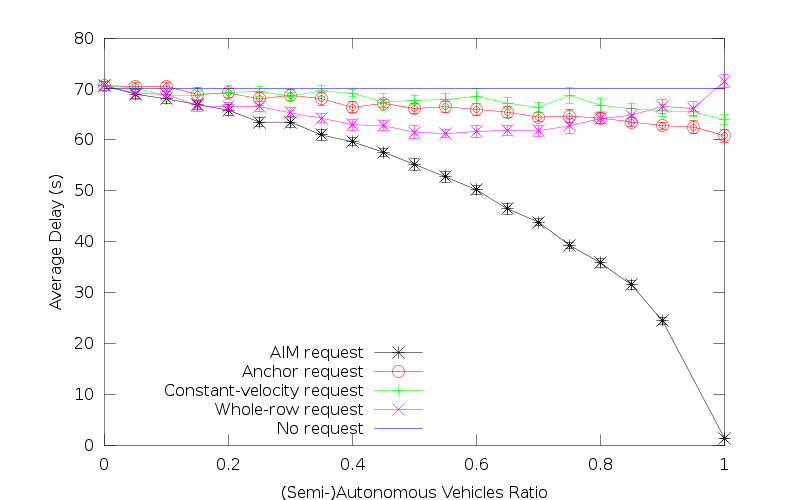
\includegraphics[width=0.8\columnwidth]{figures/figure_5.png}
\caption{Comparison on different features of semi-autonomous vehicles,
traffic level = 540 vehicles/lane/hour. Simulation time is 3600 seconds.}
\label{fig:figure5}
\end{figure}

% \commentp{If we end up with more space to use, it would be good to do
% one or two experiments along the lines of the future work mentioned in
% the last paragraph of the paper. - what happens if there are different
% amounts of traffic in different directions?}
% \commentn{This is mentioned in the future work.}


% To demonstrate the feasibility of SemiAIM as well as evaluate the
% hypothesis that SemiAIM can offer substantial improvements over
% traffic signals and FCFS-Signal, we modified the AIM4 simulator at
% \url{http://www.cs.utexas.edu/~aim} to simulate the behavior of
% vehicles in the constraint-based reservation system and measured the
% average delays of vehicles under (1) AIM, (2) SemiAIM, and (3) traffic
% signals with optimized signal timing.

% \begin{figure}[t]
%   \centering
%   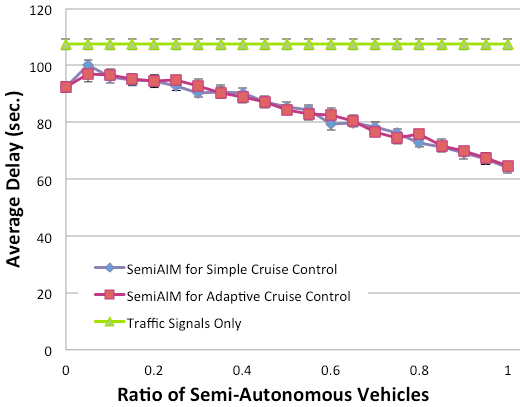
\includegraphics[width=2.4in]{figures/figure2}
%   \caption{Average delay vs. the ratio of semi-autonomous vehicles
% to human-controlled vehicles. T.
%     L. = 720 veh./hour/lane.}
%   \label{fig:figure2}
%   \vspace{-.1in}
% \end{figure}

% The experiments were conducted in a $3 \times 3$ intersection.  In the first
% experiment, the traffic consisted of human-controlled vehicles and
% fully autonomous vehicles only. We gradually increased the percentage
% of autonomous vehicles while keeping the traffic level at 720
% vehicles/hour/lane. We compared two variants of SemiAIM with optimized
% traffic signals in which all vehicles must follow the traffic signals.
% Figure~\ref{fig:figure1} shows that as the number of autonomous
% vehicles increases, the average delay decreases. In particular, when
% most vehicles are autonomous, the average delay is close to zero.  In
% the second experiment, we created a traffic consisting of
% human-controlled vehicles and two kinds of semi-autonomous vehicles
% but no autonomous vehicles.  We measured the average delay of all
% vehicles when we gradually increased the percentage of semi-autonomous
% vehicles.  Then we compared SemiAIM with optimized traffic signals.
% The results in Figure~\ref{fig:figure2} shows that as the number of
% semi-autonomous vehicles increases, the average delay decreases under
% SemiAIM.  While the decrease is not as dramatic as the decrease when
% the percentage of autonomous vehicles is near 100\% in
% Figure~\ref{fig:figure1}, SemiAIM can reduce about 43\% of the average
% delay when most vehicles are semi-autonomous.


% There are four types of
% vehicles in the simulation:
% (1) Human-Controlled Vehicles,
% (2) Semi-Autonomous Vehicles with simple cruise control,
% (3) Semi-Autonomous Vehicles with adaptive cruise control, and
% (4) Fully Autonomous Vehicles.




%%% Local Variables: 
%%% mode: latex
%%% TeX-master: "main"
%%% End:
